\documentclass{article}

\usepackage {booktabs}
\usepackage {tabularx}
\usepackage {graphicx}
\usepackage {float}

\title{Calling Bailey}
\author{ Team 5 \\ 
        William Tran \\
		Thien Trandinh \\
		Terrance Yip \\
		Susan Yuen}
\date{\today}

\begin{document}

\maketitle
\newpage
\tableofcontents
\listoffigures

\newpage

% \section {General Information}
% 
% \subsection {Terms and Definitions}
% {\renewcommand{\arraystretch}{1.4}
% \begin{tabularx}{\textwidth}{lX}
%     \toprule
% 	\textbf{Term} & \textbf{Definition} \\
% 	\midrule
%     \textbf{Node} & Another buoy. \\
% 	\bottomrule
% \end{tabularx}

\section{Module Hierarchy}
This section provides the hierarchy of the modules that will be implemented, from bottom up.

\begin{itemize}
    \item M1: Receiving Module
    \item M2: Data Processing module
    \item M3: Data Acquisition Module
    \item M4: Reply Module
\end{itemize}

\section{System Architecture}

\begin{figure}[H]
    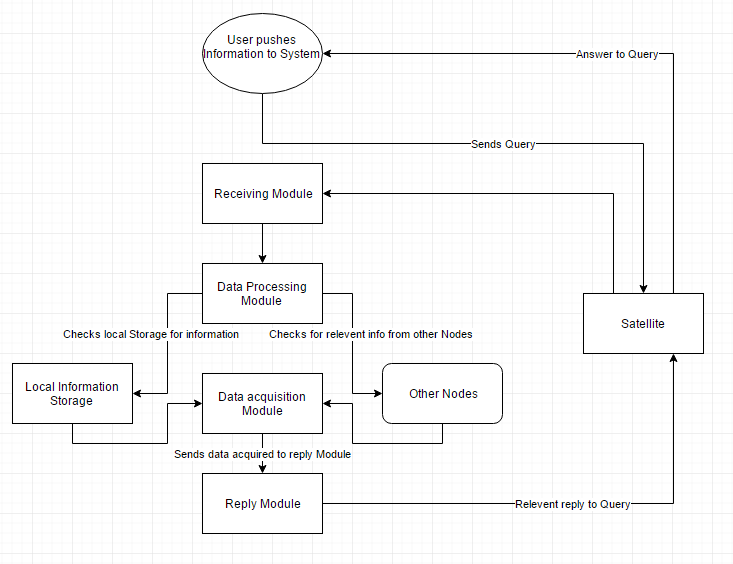
\includegraphics[width=\linewidth]{model.png}
    \caption {System Architecture}
    \label {fig:system}
\end{figure}

\section {Requirements}
\subsection{Assumptions}
The requirements for the system are based off the following assumptions:
\begin{itemize}
    \item The system receives messages from satellite phones through text messaging, and replies to the user through text messaging.
    \item All nodes contacting the system have a unique, immutable signature.
    \item The system has a reliable set of satellites that it has already established or may establish a connection to. The system is able to use these satellites to perform its duties.
    \item The weather node will update the system's weather log file.
\end{itemize}

\subsection{Functional Requirements}
\begin{enumerate}
    \item The system shall be able to take in user input through text messages.
    \item The system shall reply to the user through text messages.
    \item The system shall be able to decipher input messages into queries if possible, and shall notify the user if the message is invalid.
    \item The system shall support processing for queries of the type weather, warning, and current.
    \item For queries of type weather, the system shall reply to the user with an update of the latest weather status from the weather system.
    \item For queries of type warning, the system shall reply to the user with any warnings that have been sent within the past time period.
    \item For queries of type current, the system shall reply to the user with an update of the latest current status from the ocean current detection system.
    \item The system shall store logs for errors, weather, warnings, and ocean currents.
    \item The system shall have an option for the user to request instructions on how to use the system.
\end{enumerate}

\section {Traceability Matrices}
\subsection{Trace Between Requirements and Modules}

{\renewcommand{\arraystretch}{1.4}
\begin{tabularx}{\textwidth}{lX}
    \toprule
	\textbf{Requirements} & \textbf{Modules} \\
	\midrule
    \textbf{R1} & M1 \\
    \textbf{R2} & M4 \\
    \textbf{R3} & M2, M4 \\
    \textbf{R4} & M2 \\
    \textbf{R5} & M2, M4 \\
    \textbf{R6} & M2, M4 \\
    \textbf{R7} & M2, M4 \\
    \textbf{R8} & M3 \\
    \textbf{R9} & M1, M2, M4 \\
	\bottomrule
\end{tabularx}

\end{document}